\section{Tiered Compilation in Hotspot}
\label{sec:tiered}
As mentioned in the introduction, Programming Language Virtual Machines like Java Hotspot feature a multi-tier system when compiling methods during execution. 
Java VM's typically use Java Bytecode as input, a platform independent intermediate code generated by a Java Compiler like \texttt{javac}.
The Bytecode is meant to be interpreted by the virtual machine or further compiled into platform dependend machine code.
Hotspot includes one interpreter and two different compilers with different profiling levels resulting in a total of 5 different tiers. Since in literature and the JVM source code use the \textit{tiers} are also called \textit{compilation levels} I use both as synonyms. The following Figure \ref{f:hs_tiers} gives a short overview as well as showing the standard transitions.
\begin{figure}[ht]
  \begin{center}
    \centering
    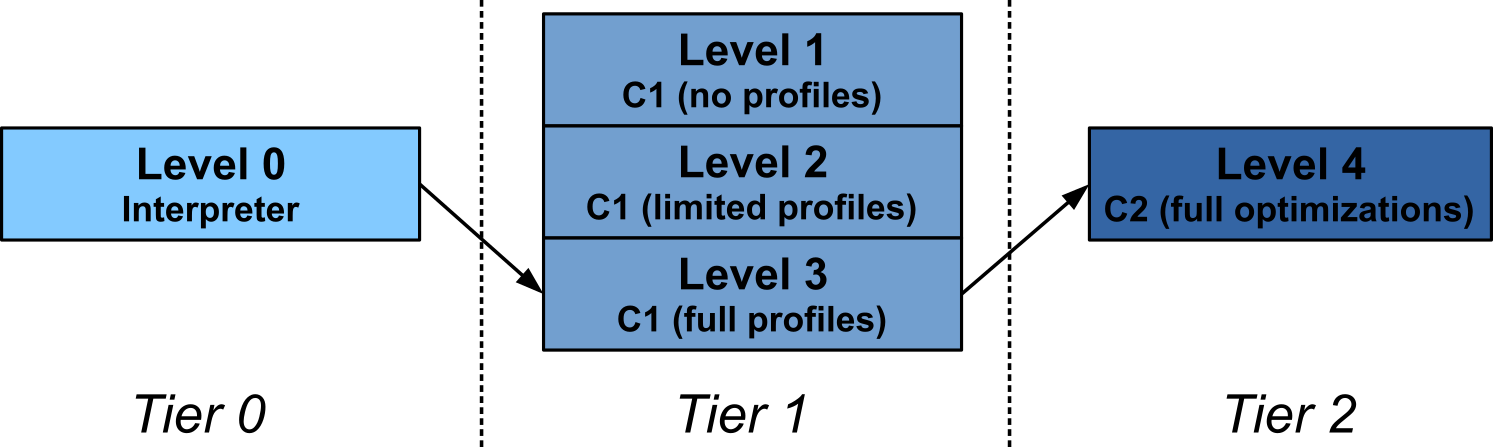
\includegraphics{figures/hs_tiers.png}
    \caption{Overview of compilation tiers}
    \label{f:hs_tiers}
  \end{center}
\end{figure}

All methods start being executed by Tier 0 also called the Interpreter.
The interpreter is template-based, meaning for each bytecode instruction it emits a predefined assembly code snippet.
During execution this code is also profiled. This means method execution counters, loop back-branches and additional statistics are counted. More importantly information about the program flow and state are gathered. These information contain for example which branches get taken or the final types of dynamically typed objects. Once one these counters exceed a predefined, constant threshold the method is considered \textit{hot} which usually results in a compilation at a higher tier.
\\\\
The standard behavior of Hotspot is to proceed with Level 3 (Tier 3). The method gets compiled with C1, also referred to as \textit{client} compiler, and continues gathering full profiles.
C1's goal is to provide a fast compilation with a low memory footprint.
The client compiler performs simple optimizations such as constant folding, null check elimination and method inlining.
More information about C1 can be found in \cite{client_compiler_talk} and \cite{client_compiler}.
The levels 1 and 2 include the same optimization but offer no or less profiling information and are used in special cases, for example if the compiler is already very busy or enough profiles are available.
\\\\
Eventually, when further compile thresholds are exceeded, the JVM further compiles the method with C2, also known as \textit{server} compiler.
The server compiler makes use of the gathered profiles in Tier 0 and Tier 3 and produces highly optimized code. C2 includes far more optimizations like loop unrolling, common subexpression elimination and elimination of range and null checks. It performs optimistic method inlining, for example by converting some virtual calls to static calls.
A more detailed look at the server compiler can be found in \cite{server_compiler}.
\\\\
The naming scheme \textit{client/server} comes from back in the days were tiered compilation was not available and one had to choose the compiler via a Hotspot command line flag. The \textit{client} compiler was meant to be used for interactive client programs with graphical user interfaces where response time is more important than peak performance. For long running server applications, the highly optimized but slower \textit{server} compiler was used. 
\\\\
Tiered compilation was introduced to improve start-up performance of the JVM.
Starting with the interpreter means that there is zero wait time until the method is executed since one does not need to wait until a compilation is finished. C1 allows the JVM to have more optimized of the code available early which then can be used to create a richer profile to be used when compiling with C2. Ideally this profile already contains most of the program flow and the assumptions made by C2 hold. If that is not the case the JVM might need to go back, gather more profiles and compile the method again. This is further described in the Section \ref{s:deoptimizations} \textit{Deoptimizations}.

\section{Deoptimizations}
\label{s:deoptimizations}
Ideally we compile a method with as much profiling information as possible.
For example, since the profiling information are usually gathered in levels 0 and 3 it can happen that a method compiled by C2 wants to execute a branch it never used before.
In this case the information about this branch are not available in the profile and therefore have not been compiled into the C2-compiled code.
This is done to allow further, very optimistic optimization and to keep the compiled code smaller. So instead, the compiler places an uncommon trap at unused branches or unloaded classes which will get triggered in case they actually get used at a later time in execution.
\\\\
The JVM then stops execution of that method and returns the control back to the interpreter. This process is called \textit{deoptimization} and considered very costly. The previous interpreter state has to be restored and the method will be executed using the slow interpreter. Eventually the method might get recompiled with the newly gained information.

\section{Compile Thresholds}
\label{s:compilethresholds}
The transitions between the compilation levels (see Fig. \ref{f:hs_tiers}) are chosen based on predefined constants called \textit{compile thresholds}. When running an instance of the JVM one can specify them manually or use the ones provided. A list of thresholds and their default values relevant to this thesis are given in Appendix \ref{a:compilethresholds}.
The standard transitions from Level 0 to 3 and 3 to 4 happen when the following predicate returns true:
\begin{align*}
& i > TierXInvocationThreshold \ * \ s \\
 || \ (&i > TierXMinInvocationThreshold \ * \ s \ \&\& \ i \ + \ b \ > \ TierXCompileThreshold \ * \ s) 
\end{align*}
where $X$ is the next compile level (3 or 4), $i$ the number of method invocations, $b$ the number of backedges and $s$ a scaling coefficient (default = 1).
The thresholds are relative and individual for interpreter and compiler.
\\\\
On Stack Replacement uses a simpler predicate:
$$b > TierXBackEdgeThreshold * s$$

Please note that there are further conditions influencing the compilation like the load on the compiler which will not be discussed.

\section{On Stack Replacement}
\label{s:onstackreplacement}
Since the JVM does not only count method invocations but also loop back branches (see also Section \ref{s:compilethresholds}) it can happen that a method gets compiled while it is still running and the compiled method is ready before the method has finished.
Instead of waiting for the next method invocation Hotspot can replace the method directly on the stack (see Figure \ref{f:osr}) and is called \textit{on stack replacement}.
An example would be a simple method consisting of a very long running loop.
\begin{figure}[ht]
  \begin{center}
    \centering
    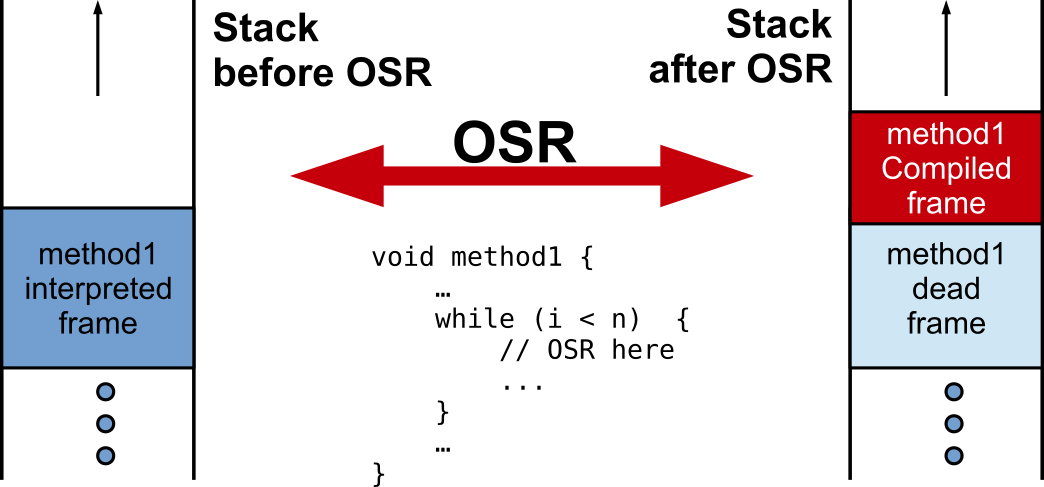
\includegraphics{figures/osr.png}
    \caption{Graphical schema of OSR}
    \label{f:osr}
  \end{center}
\end{figure}

\section{Simple Examples}

I continue with presenting two very simple examples that illustrate the usage and benefit from using cached profiles. To start I consider a standard Java Hotspot execution with OnStackReplacement disabled. I'm using my implementation described in Chapter \ref{c:implementation} in CachedProfileMode 0 (see \ref{s:mode0}).
The measurements are done on a Dual-Core machine with 8GB of RAM. To measure the method invocation time I use hprof and the average of 10 runs. The error bars show the 95\% confidence interval.
\subsection{Example 1}
\label{s:ex1}
Example one is a simple class that invokes a method one hundred times. The method itself consists of a long running loop. The source code is shown in Listing \ref{l:nocompile}.
Since OSR is disabled and a compilation to level 3 is triggered after 200 invocations this method never leaves the interpreter. I call this run the \textit{Baseline}.
To show the influence of cached profiles I use a compiler flag to lower the compile threshold explicitly and, using the functionality written for this thesis, tell Hotspot to cache the profile.
In a next execution I use these profiles and achieve significantly better performance as you can see in Figure \ref{f:nocompile}.
This increase comes mainly from the fact that having a cached profile available allows the JVM to compile methods earlier since there is no need to gather the profiling information.
\begin{lstlisting}[float,caption=Simple method that does not get compiled,label=l:nocompile,language=Java]
class NoCompile {
    double result = 0.0;
    for(int c = 0; c < 100; c++) {
      result = method1(result);
    }
    public static double method1(double count) {
        for(int k = 0; k < 10000000; k++) {
            count = count + 50000;
        }
        return count;
   }
}
\end{lstlisting}
\begin{figure}[ht]
  \begin{center}
    \centering
    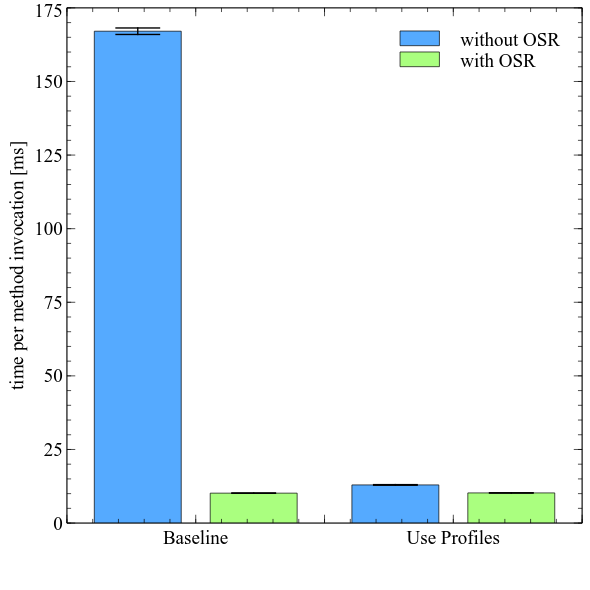
\includegraphics[width=0.5\textwidth]{figures/nocompile.png}
    \caption{NoCompile.method1 - per method invocation time}
    \label{f:nocompile}
  \end{center}
\end{figure}
\\
Enabling OSR again and the difference between with and without cached profiles vanishes.
This happens because Hotspot quickly realizes the hotness of the method and compiles it during the first invocation already. 
Since the method is simple the OSR compiled version already includes enough profiling information and does not trigger any deoptimizations. Therefore there is also no performance difference when using the cached profile.
\subsection{Example 2}
\label{s:ex2}
However, OSR is one of the main features of Hotspot to improve the JIT performance and disabling that does not give us any practical results. Since we want an example which demonstrates the influence of cached profiles, I came up with the example sketched in Listing \ref{l:manydeopts} which is slightly more complex but still easy to understand.
\\\\
The idea is to create a method that takes a different, long running branch on each of it's method invocations. Each branch has been constructed in a way that it will trigger an OSR compilation. When compiling this method during its first iteration only the first branch will be included in the compiled code. The same will happen for each of the 100 method invocations. As one can see in Figure \ref{f:manydeopts} the baseline indeed averages at around 130 deoptimizations and a time per method invocation of 200 ms.
\\\\
Now I use a regular execution to dump the profiles and then use these profiles. So theoretically the profiles dumped after a full execution should include knowledge of all branches and therefore the compiled method using these profiles should not run into any deoptimizations. As one can see in Figure \ref{f:manydeopts} this is indeed the case. When using the cached profiles no more deoptimizations occur and because less time is spent profiling and compiling the methods the per method execution time is even significantly faster with averaging at 190ms now.
\begin{lstlisting}[float,caption=Simple method that causes many deoptimizations,label=l:manydeopts,language=Java]
class ManyDeopts {
    double result = 0.0;
    for(int c = 0; c < 100; c++) {
      result = method1(result);
    }
    public static long method1(long count) {
        for(int k = 0l; k < 10000000l; k++) {
            if (count < 10000000l) {
                count = count + 1;
            } else if (count < 30000000l) {
                count = count + 2;
                .
                .
                .
            } else if (count < 50500000000l) {
               count = count + 100;
            }
            count = count + 50000;
        }
        return count;
   }
}
\end{lstlisting}
\begin{figure}[ht]
  \begin{center}
    \centering
    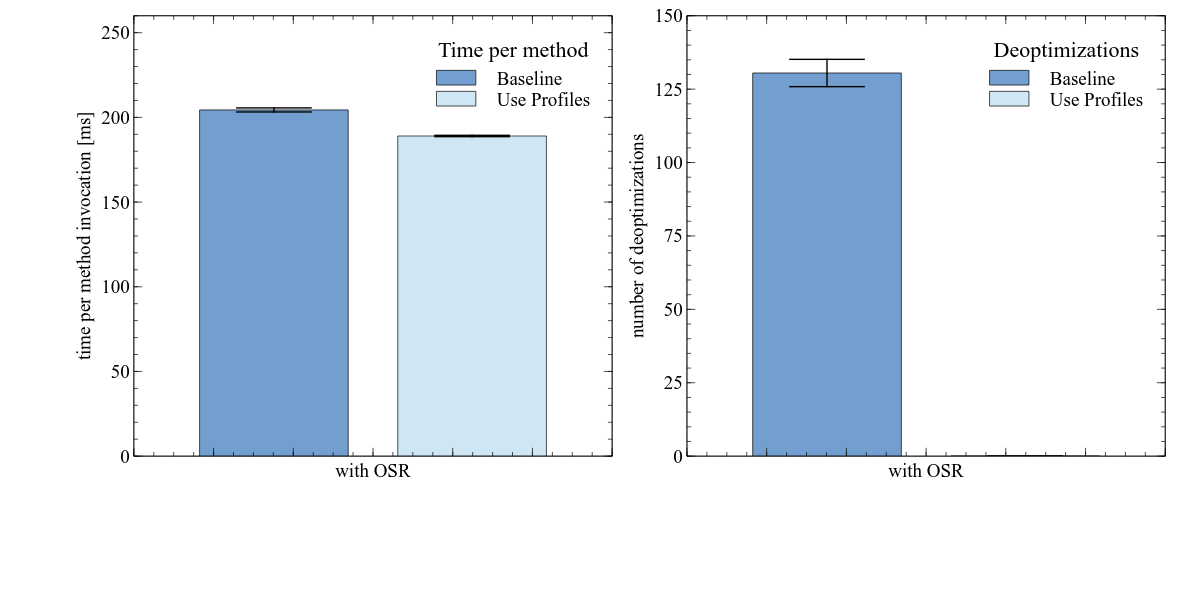
\includegraphics[width=0.9\textwidth]{figures/manydeopt.png}
    \caption{ManyDeopts.method1 - per method invocation time and deoptimization count}
    \label{f:manydeopts}
  \end{center}
\end{figure}
